\subsection{Position Across}
\label{sec:eval_req_pos_across} 

\subsubsection{Configuration}

\begin{figure}[H]
    \includegraphics[width=14cm,frame]{figures/eval_req_pos_across.png}
  \caption{Evaluation Position Across requirement}
\end{figure}

The 'Position Across' requirement is used to calculate the probability of a target report having an across-track error smaller than a defined threshold. The offset of the position (test vs. linear interpolated reference position) is used to calculate the error component across the track angle of the reference at the time. If the absolute value of this across-track position error is smaller or equal than the defined threshold, the target report is counted for the calculated probability PACOK. The PACOK must be greater or equal than the defined 'Probability' for the requirement to pass. \\

\begin{itemize}  
\item Probability [1]: Probability of acceptable across-track position
\item Probability Check Type: $\geq$
\item Maximum Absolute Value [m]: Maximum absolute across-track position difference between the test and the reference, in meters
\end{itemize}
\ \\

\subsubsection{Result Values}

\paragraph{Sector}

\begin{center}
 \begin{table}[H]
  \begin{tabularx}{\textwidth}{ | l | X |  l | }
    \hline
    \textbf{Name} & \textbf{Description} & \textbf{Example} \\ \hline
    Sector Layer & Name of the sector layer & fir\_cut\_sim \\ \hline
    Requirement Group & Name of the requirement group & Mandatory \\ \hline
    Requirement & Name of the requirement & Across \\ \hline
    Num Results & Total number of results & 728 \\ \hline
    Num Usable Results & Number of usable results & 107 \\ \hline
    Num Unusable Results & Number of unusable results & 621 \\ \hline
    Use & To be used in results & true \\ \hline
    \#Pos [1] & Number of updates & 101685 \\ \hline
    \#NoRef [1] & Number of updates w/o reference positions & 7359 \\ \hline
    \#PosInside [1] & Number of updates inside sector & 53997 \\ \hline
    \#PosOutside [1] & Number of updates outside sector & 40329 \\ \hline
    ACMin [m] & Minimum of across-track error & -444.23 \\ \hline
    ACMax [m] & Maximum of across-track error & 463.83 \\ \hline
    ACAvg [m] & Average of across-track error & 4.19 \\ \hline
    ACSDev [m] & Standard Deviation of across-track error & 24.81 \\ \hline
    ACVar [m$^2$] & Variance of across-track error & 615.60 \\ \hline
    \#ACOK [1] & Number of updates with across-track error & 52961 \\ \hline
    \#ACNOK [1] & Number of updates with unacceptable across-track error  & 1036 \\ \hline
    PACOK [\%] & Probability of acceptable across-track error & 98.08 \\ \hline
    Condition Across &  & >= 90.00 \\ \hline
    Condition Across Fulfilled &  & Passed \\ \hline
\end{tabularx}
\end{table}
\end{center}

Also, a table is given for all single targets, sorted by PACOK.

\paragraph{Single Target}

\begin{center}
 \begin{table}[H]
  \begin{tabularx}{\textwidth}{ | l | X |  l | }
    \hline
    \textbf{Name} & \textbf{Description} & \textbf{Example} \\ \hline
    Use & To be used in results & true \\ \hline
    \#Pos [1] & Number of updates & 515 \\ \hline
    \#NoRef [1] & Number of updates w/o reference positions & 45 \\ \hline
    \#PosInside [1] & Number of updates inside sector & 186 \\ \hline
    \#PosOutside [1] & Number of updates outside sector & 284 \\ \hline
    ACMin [m] & Minimum of across-track error & -28.77 \\ \hline
    ACMax [m] & Maximum of across-track error & 77.88 \\ \hline
    ACAvg [m] & Average of across-track error & 1.85 \\ \hline
    ACSDev [m] & Standard Deviation of across-track error & 12.83 \\ \hline
    ACVar [m$^2$] & Variance of across-track error & 164.55 \\ \hline
    \#ACOK [1] & Number of updates with across-track error & 185 \\ \hline
    \#ACNOK [1] & Number of updates with unacceptable across-track error  & 1 \\ \hline
    PACOK [\%] & Probability of acceptable across-track error & 99.46 \\ \hline
    Condition Across &  & >= 90.00 \\ \hline
    Condition Across Fulfilled &  & Passed \\ \hline
\end{tabularx}
\end{table}
\end{center}

\subsection{Position Along}
\label{sec:eval_req_pos_along} 

\subsubsection{Configuration}

\begin{figure}[H]
    \includegraphics[width=14cm,frame]{figures/eval_req_pos_along.png}
  \caption{Evaluation Position Along requirement}
\end{figure}

The 'Position Along' requirement is used to calculate the probability of a target report having an along-track error smaller than a defined threshold. The offset of the position (test vs. linear interpolated reference position) is used to calculate the error component along the track angle of the reference at the time. If the absolute value of this along-track position error is smaller or equal than the defined threshold, the target report is counted for the calculated probability PALOK. The PALOK must be greater or equal than the defined 'Probability' for the requirement to pass. \\

\begin{itemize}  
\item Probability [1]: Probability of acceptable along-track position
\item Probability Check Type: $\geq$
\item Maximum Absolute Value [m]: Maximum absolute along-track position difference between the test and the reference, in meters
\end{itemize}
\ \\

\subsubsection{Result Values}

\paragraph{Sector}

\begin{center}
 \begin{table}[H]
  \begin{tabularx}{\textwidth}{ | l | X |  l | }
    \hline
    \textbf{Name} & \textbf{Description} & \textbf{Example} \\ \hline
    Sector Layer & Name of the sector layer & fir\_cut\_sim \\ \hline
    Requirement Group & Name of the requirement group & Mandatory \\ \hline
    Requirement & Name of the requirement & Along \\ \hline
    Num Results & Total number of results & 728 \\ \hline
    Num Usable Results & Number of usable results & 107 \\ \hline
    Num Unusable Results & Number of unusable results & 621 \\ \hline
    Use & To be used in results & true \\ \hline
    \#Pos [1] & Number of updates & 101685 \\ \hline
    \#NoRef [1] & Number of updates w/o reference positions & 7359 \\ \hline
    \#PosInside [1] & Number of updates inside sector & 53997 \\ \hline
    \#PosOutside [1] & Number of updates outside sector & 40329 \\ \hline
    ALMin [m] & Minimum of along-track error & -1094.27 \\ \hline
    ALMax [m] & Maximum of along-track error & 828.16 \\ \hline
    ALAvg [m] & Average of along-track error & 18.37 \\ \hline
    ALSDev [m] & Standard Deviation of along-track error & 30.47 \\ \hline
    ALVar [m$^2$] & Variance of along-track error & 928.43 \\ \hline
    \#ALOK [1] & Number of updates with along-track error & 51854 \\ \hline
    \#ALNOK [1] & Number of updates with unacceptable along-track error  & 2143 \\ \hline
    PALOK [\%] & Probability of acceptable along-track error & 96.03 \\ \hline
    Condition Along &  & >= 90.00 \\ \hline
    Condition Along Fulfilled &  & Passed \\ \hline
\end{tabularx}
\end{table}
\end{center}

Also, a table is given for all single targets, sorted by PALOK.

\paragraph{Single Target}

\begin{center}
 \begin{table}[H]
  \begin{tabularx}{\textwidth}{ | l | X |  l | }
    \hline
    \textbf{Name} & \textbf{Description} & \textbf{Example} \\ \hline
    Use & To be used in results & true \\ \hline
    \#Pos [1] & Number of updates & 865 \\ \hline
    \#NoRef [1] & Number of updates w/o reference positions & 59 \\ \hline
    \#PosInside [1] & Number of updates inside sector & 482 \\ \hline
    \#PosOutside [1] & Number of updates outside sector & 324 \\ \hline
    ALMin [m] & Minimum of along-track error & -91.41 \\ \hline
    ALMax [m] & Maximum of along-track error & 100.38 \\ \hline
    ALAvg [m] & Average of along-track error & 42.52 \\ \hline
    ALSDev [m] & Standard Deviation of along-track error & 18.89 \\ \hline
    ALVar [m$^2$] & Variance of along-track error & 356.75 \\ \hline
    \#ALOK [1] & Number of updates with along-track error & 453 \\ \hline
    \#ALNOK [1] & Number of updates with unacceptable along-track error  & 29 \\ \hline
    PALOK [\%] & Probability of acceptable along-track error & 93.98 \\ \hline
    Condition Along &  & >= 90.00 \\ \hline
    Condition Along Fulfilled &  & Passed \\ \hline
\end{tabularx}
\end{table}
\end{center}

\subsection{Position Distance}
\label{sec:eval_req_pos_distance} 

\subsubsection{Configuration}

This requirement can be used in 2 variations:

\begin{figure}[H]
    \includegraphics[width=14cm,frame]{figures/eval_req_pos_distance_correct.png}
  \caption{Evaluation Position Distance requirement for correct positions}
\end{figure}

\begin{figure}[H]
    \includegraphics[width=14cm,frame]{figures/eval_req_pos_distance_false.png}
  \caption{Evaluation Position Distance requirement for false positions}
\end{figure}

The 'Position Distance' requirement is used to calculate the probability of a target report having a position error smaller or larger than a defined threshold. This two possibilities allow for calculation of a position correct or being false (e.g. outside an $5\sigma$ range of an expected error distribution). \\

The offset of the position (test vs. linear interpolated reference position) is used to calculate the Euclidean error distance. If the value of this position error fails the defined comparison threshold, the target report is counted for the calculated probability PCP (probability of check passed). The PCP must in turn pass the check for the requirement to pass. \\

The 'Failed Values are of Interest' checkbox define if the target reports passing or failing the check are of interest.


\paragraph{Position Correct Variation}

\begin{itemize}  
\item Probability [1]: Probability of correct position
\item Probability Check Type: $\geq$
\item Threshold Value [m]: Maximum allowed distance from test target report to reference
\item Threshold Value Check Type: $\leq$, distance must be less or equal the given threshold
\item Failed Values are of Interest: Checked, the distances of interest are the ones not passing the check
\end{itemize}
\ \\

\paragraph{Position False Variation}

\begin{itemize}  
\item Probability [1]: Probability of false position
\item Probability Check Type: $\leq$
\item Threshold Value [m]: Minimum distance from test target report to reference
\item Threshold Value Check Type: $\geq$, distance must be greater or equal the given threshold
\item Failed Values are of Interest: Not checked, the distances of interest are the ones passing the check
\end{itemize}
\ \\

\subsubsection{Result Values}

\paragraph{Sector}

\begin{center}
 \begin{table}[H]
  \begin{tabularx}{\textwidth}{ | l | X |  l | }
    \hline
    \textbf{Name} & \textbf{Description} & \textbf{Example} \\ \hline
    Sector Layer & Name of the sector layer & fir\_cut\_sim \\ \hline
    Requirement Group & Name of the requirement group & Mandatory \\ \hline
    Requirement & Name of the requirement & Position Correct \\ \hline
    Num Results & Total number of results & 728 \\ \hline
    Num Usable Results & Number of usable results & 107 \\ \hline
    Num Unusable Results & Number of unusable results & 621 \\ \hline
    Use & To be used in results & true \\ \hline
    \#Pos [1] & Number of updates & 101685 \\ \hline
    \#NoRef [1] & Number of updates w/o reference positions & 7359 \\ \hline
    \#PosInside [1] & Number of updates inside sector & 53997 \\ \hline
    \#PosOutside [1] & Number of updates outside sector & 40329 \\ \hline
    DMin [m] & Minimum of distance & 0.09 \\ \hline
    DMax [m] & Maximum of distance & 1115.68 \\ \hline
    DAvg [m] & Average of distance & 34.06 \\ \hline
    DSDev [m] & Standard Deviation of distance & 27.19 \\ \hline
    DVar [m$^2$] & Variance of distance & 739.18 \\ \hline
    \#CF [1] & Number of updates with failed comparison & 291 \\ \hline
    \#CP [1] & Number of updates with passed comparison  & 53706 \\ \hline
    PCP [\%] & Probability of passed comparison & 99.46 \\ \hline
    Condition &  & >= 90.00 \\ \hline
    Condition Fulfilled &  & Passed \\ \hline
\end{tabularx}
\end{table}
\end{center}

Also, a table is given for all single targets, sorted by PCP.

\paragraph{Single Target}

\begin{center}
 \begin{table}[H]
  \begin{tabularx}{\textwidth}{ | l | X |  l | }
    \hline
    \textbf{Name} & \textbf{Description} & \textbf{Example} \\ \hline
    Use & To be used in results & true \\ \hline
    \#Pos [1] & Number of updates & 927 \\ \hline
    \#NoRef [1] & Number of updates w/o reference positions & 52 \\ \hline
    \#PosInside [1] & Number of updates inside sector & 646 \\ \hline
    \#PosOutside [1] & Number of updates outside sector & 229 \\ \hline
    DMin [m] & Minimum of distance & 4.14 \\ \hline
    DMax [m] & Maximum of distance & 284.87 \\ \hline
    DAvg [m] & Average of distance & 81.87 \\ \hline
    DSDev [m] & Standard Deviation of distance & 34.43 \\ \hline
    DVar [m$^2$] & Variance of distance & 1185.18 \\ \hline
    \#CF [1] & Number of updates with failed comparison & 25 \\ \hline
    \#CP [1] & Number of updates with  passed comparison & 621 \\ \hline
    PCP [\%] & Probability of passed comparison & 96.13 \\ \hline
    Condition &  & >= 90.00 \\ \hline
    Condition Fulfilled &  & Passed \\ \hline
\end{tabularx}
\end{table}
\end{center}

\subsection{Position Distance RMS}
\label{sec:eval_req_pos_distance_rms} 

\subsubsection{Configuration}

\begin{figure}[H]
    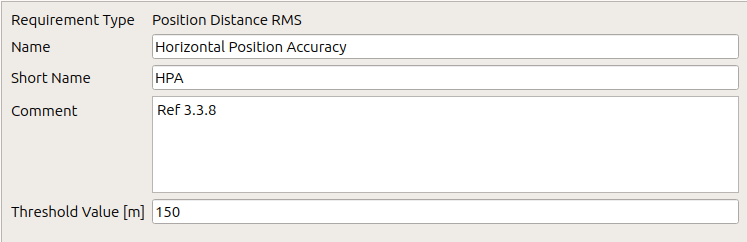
\includegraphics[width=14cm,frame]{figures/eval_req_pos_distance_rms.png}
  \caption{Evaluation Position Latency requirement}
\end{figure}

The 'Position Distance' requirement is used to calculate if the RMS position error is larger than a defined threshold. \\

The offset of the position (test vs. linear interpolated reference position) is used to calculate the RMS error distance for a number of target reports. The requirement is failed if the the calculated RMS value is larger than the defined threshold. \\

\begin{itemize}  
\item Threshold Value [m]: Maximum allowed RMS
\end{itemize}

\subsubsection{Result Values}

\paragraph{Sector}

\begin{center}
 \begin{table}[H]
  \begin{tabularx}{\textwidth}{ | l | X |  l | }
    \hline
    \textbf{Name} & \textbf{Description} & \textbf{Example} \\ \hline
    Sector Layer & Name of the sector layer & fir\_cut\_sim \\ \hline
    Requirement Group & Name of the requirement group & Mandatory \\ \hline
    Requirement & Name of the requirement & Position Correct \\ \hline
    Num Results & Total number of results & 728 \\ \hline
    Num Usable Results & Number of usable results & 107 \\ \hline
    Num Unusable Results & Number of unusable results & 621 \\ \hline
    Use & To be used in results & true \\ \hline
    \#Pos [1] & Number of updates & 101685 \\ \hline
    \#NoRef [1] & Number of updates w/o reference positions & 7359 \\ \hline
    \#PosInside [1] & Number of updates inside sector & 53997 \\ \hline
    \#PosOutside [1] & Number of updates outside sector & 40329 \\ \hline
    DMin [m] & Minimum of distance & 0.23 \\ \hline
    DMax [m] & Maximum of distance & 515.87 \\ \hline
    DAvg [m] & Average of distance & 29.25 \\ \hline
    DSDev [m] & Standard Deviation of distance & 23.12 \\ \hline
    DVar [$m^2$] & Variance of distance & 534.32 \\ \hline
    RMS & Root mean square & 37.28 \\ \hline
    \#CF [1] & Number of updates with failed comparison & 9 \\ \hline
    \#CP [1] & Number of updates with passed comparison  & 33234 \\ \hline
    Condition &  & <= 350.000000 \\ \hline
    Condition Fulfilled &  & Passed \\ \hline
\end{tabularx}
\end{table}
\end{center}

Also, a table is given for all single targets, sorted by RMS.

\paragraph{Single Target}

\begin{center}
 \begin{table}[H]
  \begin{tabularx}{\textwidth}{ | l | X |  l | }
    \hline
    \textbf{Name} & \textbf{Description} & \textbf{Example} \\ \hline
    Use & To be used in results & true \\ \hline
    \#Pos [1] & Number of updates & 927 \\ \hline
    \#NoRef [1] & Number of updates w/o reference positions & 52 \\ \hline
    \#PosInside [1] & Number of updates inside sector & 646 \\ \hline
    \#PosOutside [1] & Number of updates outside sector & 229 \\ \hline
    DMin [m] & Minimum of distance & 58.89 \\ \hline
    DMax [m] & Maximum of distance & 371.66 \\ \hline
    DAvg [m] & Average of distance & 110.69 \\ \hline
    DSDev [m] & Standard Deviation of distance & 59.38 \\ \hline
    DVar [$m^2$] & Variance of distance & 125.61 \\ \hline
    RMS & Root mean square & 3525.42 \\ \hline
    \#CF [1] & Number of updates with failed comparison & 1 \\ \hline
    \#CP [1] & Number of updates with passed comparison & 31 \\ \hline
    Condition &  & <= 350.000000 \\ \hline
    Condition Fulfilled &  & Passed \\ \hline
\end{tabularx}
\end{table}
\end{center}

\subsection{Position Latency}
\label{sec:eval_req_pos_latency} 

\subsubsection{Configuration}

\begin{figure}[H]
    \includegraphics[width=14cm,frame]{figures/eval_req_pos_latency.png}
  \caption{Evaluation Position Latency requirement}
\end{figure}

The 'Position Latency' requirement is used to calculate the probability of a target report having a time-latency error smaller than a defined threshold. The offset of the position (test vs. linear interpolated reference position) is used to calculate the error component along the track angle of the reference at the time, which divided by the negative speed gives the latency. If the absolute value of this latency is smaller or equal than the defined threshold, the target report is counted for the calculated probability PLTOK. The PLTOK must be greater or equal than the defined 'Probability' for the requirement to pass. \\

\begin{itemize}  
\item Probability [1]: Probability of acceptable position latency
\item Probability Check Type: $\geq$
\item Maximum Absolute Value [s]: Maximum absolute latency, in seconds
\end{itemize}
\ \\

\subsubsection{Result Values}

\paragraph{Sector}

\begin{center}
 \begin{table}[H]
  \begin{tabularx}{\textwidth}{ | l | X |  l | }
    \hline
    \textbf{Name} & \textbf{Description} & \textbf{Example} \\ \hline
    Sector Layer & Name of the sector layer & fir\_cut\_sim \\ \hline
    Requirement Group & Name of the requirement group & Mandatory \\ \hline
    Requirement & Name of the requirement & Latency \\ \hline
    Num Results & Total number of results & 728 \\ \hline
    Num Usable Results & Number of usable results & 107 \\ \hline
    Num Unusable Results & Number of unusable results & 621 \\ \hline
    Use & To be used in results & true \\ \hline
    \#Pos [1] & Number of updates & 101685 \\ \hline
    \#NoRef [1] & Number of updates w/o reference positions & 7359 \\ \hline
    \#PosInside [1] & Number of updates inside sector & 53997 \\ \hline
    \#PosOutside [1] & Number of updates outside sector & 40329 \\ \hline
    LTMin [s] & Minimum of latency & -00:00:02.758 \\ \hline
    LTMax [s] & Maximum of latency & 00:00:04.790 \\ \hline
    LTAvg [s] & Average of latency & -00:00:00.081 \\ \hline
    LTSDev [s] & Standard Deviation of latency & 00:00:00.146 \\ \hline
    LTVar [s$^2$] & Variance of latency & 00:00:00.021 \\ \hline
    \#LTOK [1] & Number of updates with latency & 44216 \\ \hline
    \#LTNOK [1] & Number of updates with unacceptable latency  & 9781 \\ \hline
    PLTOK [\%] & Probability of acceptable latency & 81.89 \\ \hline
    Condition Latency &  & >= 90.00 \\ \hline
    Condition Latency Fulfilled &  & Failed \\ \hline
\end{tabularx}
\end{table}
\end{center}

Also, a table is given for all single targets, sorted by PLTOK.

\paragraph{Single Target}

\begin{center}
 \begin{table}[H]
  \begin{tabularx}{\textwidth}{ | l | X |  l | }
    \hline
    \textbf{Name} & \textbf{Description} & \textbf{Example} \\ \hline
    Use & To be used in results & true \\ \hline
    \#Pos [1] & Number of updates & 1729 \\ \hline
    \#NoRef [1] & Number of updates w/o reference positions & 142 \\ \hline
    \#PosInside [1] & Number of updates inside sector & 1469 \\ \hline
    \#PosOutside [1] & Number of updates outside sector & 118 \\ \hline
    LTMin [s] & Minimum of latency & -00:00:00.590 \\ \hline
    LTMax [s] & Maximum of latency & 00:00:00.431 \\ \hline
    LTAvg [s] & Average of latency & -00:00:00.092 \\ \hline
    LTSDev [s] & Standard Deviation of latency & 00:00:00.085 \\ \hline
    LTVar [s$^2$] & Variance of latency & 00:00:00.007 \\ \hline
    \#LTOK [1] & Number of updates with latency & 1324 \\ \hline
    \#LTNOK [1] & Number of updates with unacceptable latency  & 145 \\ \hline
    PLTOK [\%] & Probability of acceptable latency & 90.13 \\ \hline
    Condition Latency &  & >= 90.00 \\ \hline
    Condition Latency Fulfilled &  & Passed \\ \hline
\end{tabularx}
\end{table}
\end{center}


%
\subsection{Position Radar Azimuth}
\label{sec:eval_req_pos_radar_azm} 

\subsubsection{Configuration}

\begin{figure}[H]
    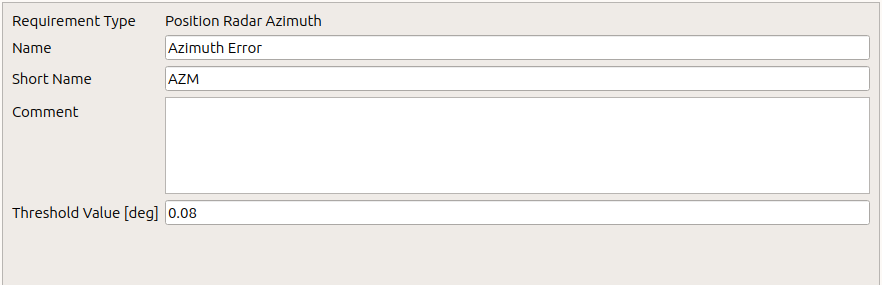
\includegraphics[width=14cm,frame]{figures/eval_req_pos_radar_azm.png}
  \caption{Evaluation Position Radar Azimuth requirement}
\end{figure}

The ’Position Radar Azimuth requirement is used to calculate the probability of a target report
having an Radar azimuth error smaller than a defined threshold. The offset of the position
(test vs. linear interpolated reference position) is used to calculate the azimuth error component
w.r.t. the respective Radar. If the absolute value of this range
position error is smaller or equal than the defined threshold, the target report is counted
for the calculated probability CP. The CP must be greater or equal than the
defined ’Probability’ for the requirement to pass.
\ \\

\begin{itemize}  
\item Maximum Absolute Value [m]: Maximum azimuth offset allowed 
\end{itemize}

\subsubsection{Result Values}

\paragraph{Sector}

\begin{center}
 \begin{table}[H]
  \begin{tabularx}{\textwidth}{ | l | X |  l | }
    \hline
    \textbf{Name} & \textbf{Description} & \textbf{Example} \\ \hline
  Sector Layer & Name of the sector layer & DOI  \\ \hline
  Requirement Group & Name of the requirement group & Test  \\ \hline
  Requirement & Name of the requirement & Azimuth Error  \\ \hline
  Num Results & Total number of results & 368  \\ \hline
  Num Usable Results & Number of usable results & 136  \\ \hline
  Num Unusable Results & Number of unusable results & 232  \\ \hline
  Use & To be used in results & true  \\ \hline
  \#Pos [1] & Number of updates & 28705  \\ \hline
  \#NoRef [1] & Number of updates w/o reference positions & 12861  \\ \hline
  \#PosInside [1] & Number of updates inside sector & 15113  \\ \hline
  \#PosOutside [1] & Number of updates outside sector & 731  \\ \hline
  DMin [m] & Minimum of angle distance & -103.90  \\ \hline
  DMax [m] & Maximum of angle distance & 28.27  \\ \hline
  DAvg [m] & Average of angle distance & -0.01  \\ \hline
  DSDev [m] & Standard Deviation of angle distance & 1.25  \\ \hline
  DVar [$m^2$] & Variance of angle distance & 1.57  \\ \hline
  \#CF [1] & Number of updates with failed comparison & 1860  \\ \hline
  \#CP [1] & Number of updates with passed comparison  & 13253  \\ \hline
  Condition &  & <= 0.080000  \\ \hline
  Condition Fulfilled &  & Passed  \\ \hline
\end{tabularx}
\end{table}
\end{center}

Also, a table is given for all single targets, sorted by \#CF.

\paragraph{Single Target}

\begin{center}
 \begin{table}[H]
  \begin{tabularx}{\textwidth}{ | l | X |  l | }
    \hline
    \textbf{Name} & \textbf{Description} & \textbf{Example} \\ \hline
    Use & To be used in results & true \\ \hline
    \#Pos [1] & Number of updates & 394 \\ \hline
    \#NoRef [1] & Number of updates w/o reference positions & 72 \\ \hline
    \#PosInside [1] & Number of updates inside sector & 285 \\ \hline
    \#PosOutside [1] & Number of updates outside sector & 37 \\ \hline
    DMin [m] & Minimum of angle distance & -0.02 \\ \hline
    DMax [m] & Maximum of angle distance & 0.15 \\ \hline
    DAvg [m] & Average of angle distance & 0.09 \\ \hline
    DSDev [m] & Standard Deviation of angle distance & 0.03 \\ \hline
    DVar [$m^2$] & Variance of angle distance & 0.00 \\ \hline
    \#CF [1] & Number of updates with failed comparison & 191 \\ \hline
    \#CP [1] & Number of updates with passed comparison & 94 \\ \hline
    Condition &  & <= 0.080000 \\ \hline
    Condition Fulfilled &  & Passed \\ \hline
\end{tabularx}
\end{table}
\end{center}


\subsection{Position Radar Range}
\label{sec:eval_req_pos_radar_rng} 

\subsubsection{Configuration}

\begin{figure}[H]
    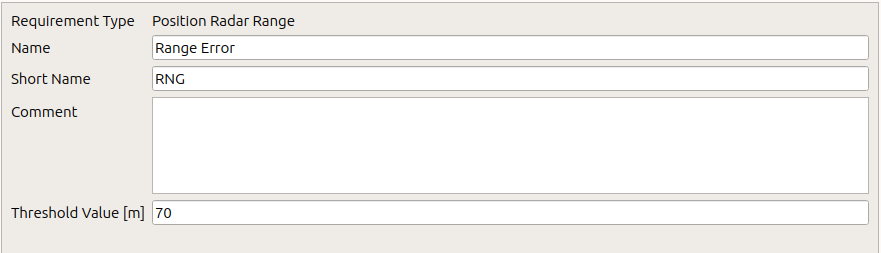
\includegraphics[width=14cm,frame]{figures/eval_req_pos_radar_rng.png}
  \caption{Evaluation Position Radar Range requirement}
\end{figure}

The ’Position Radar Range’ requirement is used to calculate the probability of a target report
having an Radar range error smaller than a defined threshold. The offset of the position
(test vs. linear interpolated reference position) is used to calculate the range error component
w.r.t. the respective Radar. If the absolute value of this range
position error is smaller or equal than the defined threshold, the target report is counted
for the calculated probability CP. The CP must be greater or equal than the
defined ’Probability’ for the requirement to pass.
\ \\

\begin{itemize}  
\item Maximum Absolute Value [m]: Maximum range offset allowed 
\end{itemize}

\subsubsection{Result Values}

\paragraph{Sector}

\begin{center}
 \begin{table}[H]
  \begin{tabularx}{\textwidth}{ | l | X |  l | }
    \hline
    \textbf{Name} & \textbf{Description} & \textbf{Example} \\ \hline
  Sector Layer & Name of the sector layer & DOI \\ \hline
  Requirement Group & Name of the requirement group & Test \\ \hline
  Requirement & Name of the requirement & Range Error \\ \hline
  Num Results & Total number of results & 368 \\ \hline
  Num Usable Results & Number of usable results & 136 \\ \hline
  Num Unusable Results & Number of unusable results & 232 \\ \hline
  Use & To be used in results & true \\ \hline
  \#Pos [1] & Number of updates & 28705 \\ \hline
  \#NoRef [1] & Number of updates w/o reference positions & 12861 \\ \hline
  \#PosInside [1] & Number of updates inside sector & 15113 \\ \hline
  \#PosOutside [1] & Number of updates outside sector & 731 \\ \hline
  DMin [m] & Minimum of distance & -25389.26 \\ \hline
  DMax [m] & Maximum of distance & 3216.65 \\ \hline
  DAvg [m] & Average of distance & 15.11 \\ \hline
  DSDev [m] & Standard Deviation of distance & 216.87 \\ \hline
  DVar [$m^2$] & Variance of distance & 47034.17 \\ \hline
  \#CF [1] & Number of updates with failed comparison & 1613 \\ \hline
  \#CP [1] & Number of updates with passed comparison  & 13500 \\ \hline
  Range Bias [m] & Range bias (linear estimation) & -1.42 \\ \hline
  Range Gain [1] & Range gain (linear estimation) & 1.00014 \\ \hline
  Condition &  & <= 70.000000 \\ \hline
  Condition Fulfilled &  & Passed \\ \hline

\end{tabularx}
\end{table}
\end{center}

Also, a table is given for all single targets, sorted by \#CF.

\paragraph{Single Target}

\begin{center}
 \begin{table}[H]
  \begin{tabularx}{\textwidth}{ | l | X |  l | }
    \hline
    \textbf{Name} & \textbf{Description} & \textbf{Example} \\ \hline
    Use & To be used in results & true \\ \hline
    \#Pos [1] & Number of updates & 18 \\ \hline
    \#NoRef [1] & Number of updates w/o reference positions & 0 \\ \hline
    \#PosInside [1] & Number of updates inside sector & 18 \\ \hline
    \#PosOutside [1] & Number of updates outside sector & 0 \\ \hline
    DMin [m] & Minimum of distance & -246.29 \\ \hline
    DMax [m] & Maximum of distance & -2.50 \\ \hline
    DAvg [m] & Average of distance & -19.56 \\ \hline
    DSDev [m] & Standard Deviation of distance & 55.05 \\ \hline
    DVar [$m^2$] & Variance of distance & 0.00 \\ \hline
    Range Bias [m] & Range bias (linear estimation) & 43520.69 \\ \hline
    Range Gain [1] & Range gain (linear estimation) & 0.80278 \\ \hline
    \#CF [1] & Number of updates with failed comparison & 1 \\ \hline
    \#CP [1] & Number of updates with passed comparison & 17 \\ \hline
    Condition &  & <= 70.000000 \\ \hline
    Condition Fulfilled &  & Passed \\ \hline
\end{tabularx}
\end{table}
\end{center}
